% Created 2017-03-12 Sun 14:53
% Intended LaTeX compiler: pdflatex
\documentclass[presentation]{beamer}
\usepackage[utf8]{inputenc}
\usepackage[T1]{fontenc}
\usepackage{graphicx}
\usepackage{grffile}
\usepackage{longtable}
\usepackage{wrapfig}
\usepackage{rotating}
\usepackage[normalem]{ulem}
\usepackage{amsmath}
\usepackage{textcomp}
\usepackage{amssymb}
\usepackage{capt-of}
\usepackage{hyperref}
\usetheme{CambridgeUS}
\usecolortheme{beaver}
\setcounter{secnumdepth}{1}
\author{Zheng Tian}
\date{}
\title{Lecture 6: Linear Regression with One Regressor}
\hypersetup{
 pdfauthor={Zheng Tian},
 pdftitle={Lecture 6: Linear Regression with One Regressor},
 pdfkeywords={},
 pdfsubject={},
 pdfcreator={Emacs 25.1.1 (Org mode 9.0.3)},
 pdflang={English}}
\begin{document}

\maketitle
\begin{frame}{Outline}
\setcounter{tocdepth}{1}
\tableofcontents
\end{frame}


\section{The Linear Regression Model}
\label{sec:org80d75fe}

\begin{frame}[label={sec:org3532a4e}]{Definition of \alert{regress} in Merriam-Webster's dictionary}
Merriam-Webster gives the following definition of the word "regress":
\begin{enumerate}
\item An act or the privilege of going or coming back
\item Movement backward to a previous and especially worse or more
primitive state or condition
\item The act of reasoning backward
\end{enumerate}
\end{frame}

\begin{frame}[label={sec:org1b079e3}]{The meaning of regression in statistics?}
\begin{itemize}
\item In statistics, regression analysis focus on the conditional mean of the
dependent variable given the independent variables, which is a
function of the values of independent variables.

\item A very simple functional form of a conditional expectation is a linear
function. That is, we can model the conditional mean as follows,

\begin{equation}
\label{eq:genpopreg}
\mathrm{E}(Y \mid X = x) = f(x) = \beta_{0} + \beta_1 x
\end{equation}

The above equation is a \alert{simple linear regression function}.
\end{itemize}
\end{frame}

\begin{frame}[label={sec:org79efb0f}]{Research question:}
\begin{quote}
The research question of this application is: Can reducing class size
increase students' test scores?
\end{quote}

\begin{itemize}
\item How can we answer this question?
\end{itemize}
\end{frame}

\begin{frame}[label={sec:orgacb6531}]{Randomized controlled experiment}
\begin{itemize}
\item Randomly choose 42 students and divide them into two classes,
with one having 20 students and another having 22.
\item They are
taught with the same subject and by the same teachers.
\item Randomization ensures that it is the difference in class sizes of
the two classes that is the only factor affecting test scores.
\end{itemize}
\end{frame}

\begin{frame}[label={sec:org2636fbc}]{Compute conditional means}
\begin{itemize}
\item After a test for both classes, we then compute the expected values
of test scores, given the different class sizes.
\begin{gather*}
\mathrm{E}(TestScore | ClassSize = 20) \\
\mathrm{E}(TestScore | ClassSize = 22)
\end{gather*}

\item Then the effect of class size on test scores is the difference in
the conditional means, i.e.,
\begin{equation*}
\mathrm{E}(TestScore | ClassSize = 20) - \mathrm{E}(TestScore | ClassSize = 22)
\end{equation*}
\end{itemize}
\end{frame}

\begin{frame}[label={sec:org6973932}]{The population regression function for test scores on class sizes}
\begin{itemize}
\item We use a linear regression function to describe the relationship
between test scores and class sizes.

\item The \alert{population regression function} or the \alert{population regression
line}

\begin{equation}
\label{eq:popreg-testscore}
\mathrm{E}(TestScore | ClassSzie) = \beta_0 + \beta_1 ClassSize
\end{equation}
\end{itemize}
\end{frame}

\begin{frame}[label={sec:org18215b5}]{The simple linear regression model for test scores on class sizes}
\begin{itemize}
\item We can lump all these factors into a single term, and set up a \alert{simple linear
regression model} as follows,

\begin{equation}
\label{eq:regmodel-testscore}
TestScore = \beta_0 + \beta_1 ClassSize + OtherFactors
\end{equation}

\item If we assume \(\mathrm{E}(OtherFactors | ClassSize) = 0\), then the
simple linear regression model becomes the population regression line.
\end{itemize}
\end{frame}

\begin{frame}[label={sec:org48e72a0}]{A distinction between the population regression function and the population regression model}
\begin{itemize}
\item A population regression function
\begin{itemize}
\item It's a deterministic relation between class size and the expectation of
test scores.
\item However, we cannot compute the exact value of the test score of a
particular observation.
\end{itemize}

\item A population regression model
\begin{itemize}
\item It's a complete description of a data generating process (DGP).
\item The association between test scores and class size is not
deterministic, depending on the value of other factors.
\end{itemize}
\end{itemize}
\end{frame}

\begin{frame}[label={sec:org254d59c}]{An interpretation of the population regression model}
\begin{itemize}
\item Now we have set up the simple linear regression model,
\begin{equation*}
TestScore = \beta_0 + \beta_1 ClassSize + OtherFactors
\end{equation*}
What is \(\beta_1\) and \(\beta_0\) represent in the model?
\end{itemize}
\end{frame}

\begin{frame}[label={sec:org555890e}]{Interpret \(\beta_1\)}
\begin{itemize}
\item Denote \(\Delta TestScore\) and \(\Delta ClassSize\) to
be their respective change.

\item \alert{Holding other factors constant}, we have
\[ \Delta TestScore = \beta_1 \Delta ClassSize  \]
where \(\beta_0\) is removed because it is also a constant.

\item Then, we get

\[ \beta_1 = \frac{\Delta TestScore}{\Delta ClassSize} \]

That is, \(\beta_1\) measures the change in the test score resulting
from a \alert{one-unit change} in the class size.
\end{itemize}
\end{frame}

\begin{frame}[label={sec:org166f572}]{Marginal effect}
\begin{itemize}
\item When \(TestScore\) and
\(ClassSize\) are two continuous variable, we can write \(\beta_1\) as

\[\beta_1 = \frac{\mathrm{d} TestScore}{\mathrm{d} ClassSize}  \]

\item We often call \(\beta_1\) as the \alert{marginal effect} of the class
size on the test score.
\end{itemize}
\end{frame}

\begin{frame}[label={sec:orgb35c3fc}]{Holding other things constant}
\begin{itemize}
\item The phrase of "holding other factors constant" is important. Without
it, we cannot disentangle the effect of class sizes on test scores
from other factors.
\item "Holding other things constant" is often expressed
as the notion of \alert{ceteris paribus}.
\end{itemize}
\end{frame}

\begin{frame}[label={sec:org40b83a7}]{Interpret \(\beta_0\)}
\begin{itemize}
\item \(\beta_0\) is the intercept in the model.
\item Sometimes it bears real
meanings, but sometimes it merely presents as an intercept.
\item In regression model of test scores on class sizes, \(\beta_0\) is the
test score when the class size and other factors are all zero, which
is obviously nonsensical.
\end{itemize}
\end{frame}

\begin{frame}[label={sec:orga3225e4}]{The general linear regression model}
\begin{itemize}
\item Consider two random variables \(Y\) and \(X\). For both, there are \(n\) observations so that
each observation \(i = 1, 2, 3, \ldots\) is associated with a pair of
values of \((X_i, Y_i)\).

\item Then a \alert{simple linear regression model} that associates \(Y\) with \(X\) is

\begin{equation}
\label{eq:single-regress}
Y_i = \beta_0 + \beta_1 X_i + u_i, \text{ for } i = 1, \ldots, n
\end{equation}

\item \(Y_i\) is called the dependent variable, the regressand, or the LHS
(left-hand side) variable.
\item \(X_i\) is called the independent variable, the regressor, or the RHS
(right-hand side) variable.
\end{itemize}
\end{frame}

\begin{frame}[label={sec:org9eae4ee}]{The general linear regression model (cont'd)}
\begin{itemize}
\item \(\beta_{0}\) is the intercept, or the constant term. It can either have
economic meaning or have merely mathematical sense, which determines
the level of the regression line, i.e., the point of intersection
with the Y axis.
\item \(\beta_{1}\) is the slope of the population regression line. Since
\(\beta_1 = \mathrm{d}Y_i/ \mathrm{d}X_i\), it is the marginal effect
of \(X\) on \(Y\). That is, holding other things constant, one unit
change in \(X\) will make \(Y\) change by \(\beta_1\) units.
\item \(u_i\) is the error term. \(u_i = Y_i - (\beta_0 + \beta_1 X_i)\)
incorporates all the other factors besides \(X\) that determine the
value of \(Y\).
\item \(\beta_{0} + \beta_{1}X_{i}\) represents the population regression
function(or the population regression line).
\end{itemize}
\end{frame}

\begin{frame}[label={sec:org57cf958}]{An graphical illustration of a linear regression model}
\begin{figure}[htbp]
\centering
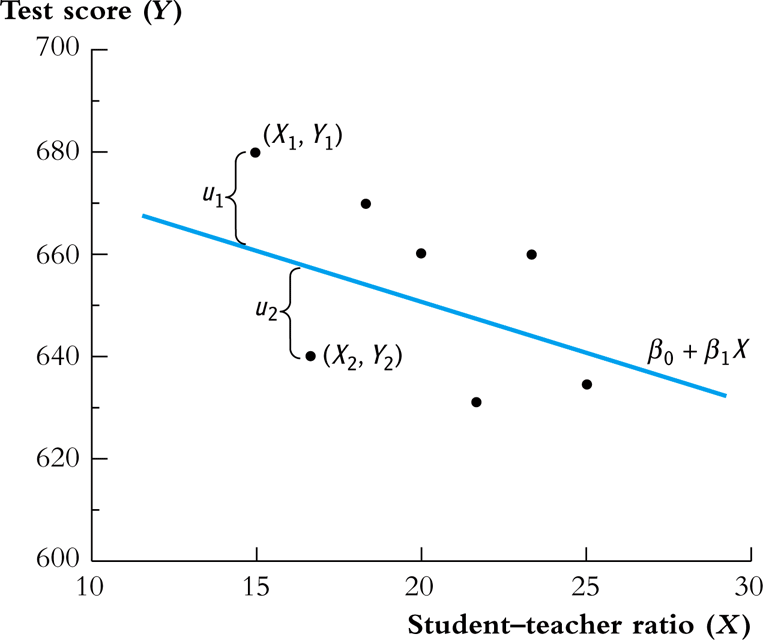
\includegraphics[width=0.75\textwidth]{figure/fig-4-1.png}
\caption{\label{fig:orgf424c3a}
The Population Regression Line}
\end{figure}
\end{frame}
\end{document}